\section{Model}
\label{sec:model}

The basic element of our model is a \tg, which represents a graph that
evolves over time.  We define the structure of an evolving graph in
Section~\ref{sec:model:structure}.  We then show the relationship with
other models in Section~\ref{sec:model:others}.  Finally, in
Section~\ref{sec:model:algebra} we define the algebraic operations on
our model.

\subsection{Evolving Graphs}
\label{sec:model:structure}

First we describe how time is represented in our model.  Following the
SQL:2011 standard~\cite{DBLP:journals/sigmod/KulkarniM12}, we adopt
the {\em closed-open} period model, where a period represents all
times starting from and including the start time, continuing to but
excluding the end time.

\begin{definition}[Time period]
A {\em time period} \\$p = [start, end)$ is an interval on the
  continuous time domain $T$, subject to the constraint $start < end$.
\label{def:period} 
\end{definition}

\begin{definition}[TGraph]
An {\em evolving graph} $TG$ is a pair $(V;E)$, where $V$ is a finite
set of nodes with schema $(\underline{vid}, a_1, \ldots, a_n,
\underline{p})$, and $E$ is a finite set of edges connecting pairs of
nodes from $V$, with schema $(\underline{vid_1}, \underline{vid_2},
b_1, \ldots, b_m, \underline{p})$, and $p$ is a {\em maximally
  coalesced} time period.  Formally stated, the relationship between
$V$ and $E$ is through a constraint on $E$: $\forall e(vid_1, vid_2,
p_i) \in E, \exists v1(vid_1, p_j)$ and $v2(vid_2, p_k)$ and
$p_i.contains(p_j)$ and $p_i.contains(p_k)$.
\label{def:tg}
\end{definition}

The time periods of all graph entities, i.e. vertices and edges, are
maximally coalesced.  That means that all the tuples in $V$ and $E$
are distinct in all attributes, including the time periods, and that
time periods do not overlap for any individual entity.  The above
evolving graph definition~\ref{def:tg} can be expressed in temporal
SQL as follows (without attributes):

\begin{small}
\begin{verbatim}
CREATE TABLE V (
  vid LONG,
  estart DATE,
  eend DATE,
  PERIOD for eperiod (estart, eend),
  PRIMARY KEY (vid, eperiod WITHOUT OVERLAPS)
);
CREATE TABLE E (
  vid1 LONG,
  vid2 LONG,
  estart DATE,
  eend DATE,
  PERIOD for eperiod (estart, eend),
  PRIMARY KEY (vid1, vid2, eperiod WITHOUT OVERLAPS),
  FOREIGN KEY (vid1, PERIOD eperiod) REFERENCES V(vid, PERIOD eperiod),
  FOREIGN KEY (vid2, PERIOD eperiod) REFERENCES V(vid, PERIOD eperiod)
)
\end{verbatim}
\end{small}

\vera{placeholder for schema on load explanation}

\subsection{Other Models}
\label{sec:model:other}

Most commonly an evolving graph is considered to be a sequence of
graph snapshots corresponding to time instances in the discreet time
domain $T$ (\cite{Khurana2013,DBLP:journals/tos/MiaoHLWYZPCC15}).
Such a model has point semantics on the time domain.  Point semantics
has several limitations:

\begin{itemize}[noitemsep,topsep=0pt]
\item It requires a discreet time domain.  The state of the graph can
  be undefined at some time $t_i$ unless a snapshot is associated with
  each possible value of $T$ in the discreet range $[t_{start}, now)$.
\item It is not compact.  Every change to an entity (vertex or edge)
  requires a new snapshot.  For large graphs, consecutive snapshots
  have degree of similarity approaching 1 (on the scale of 0 of no
  similarity and 1 full similarity).
\end{itemize}

\begin{figure}[h]
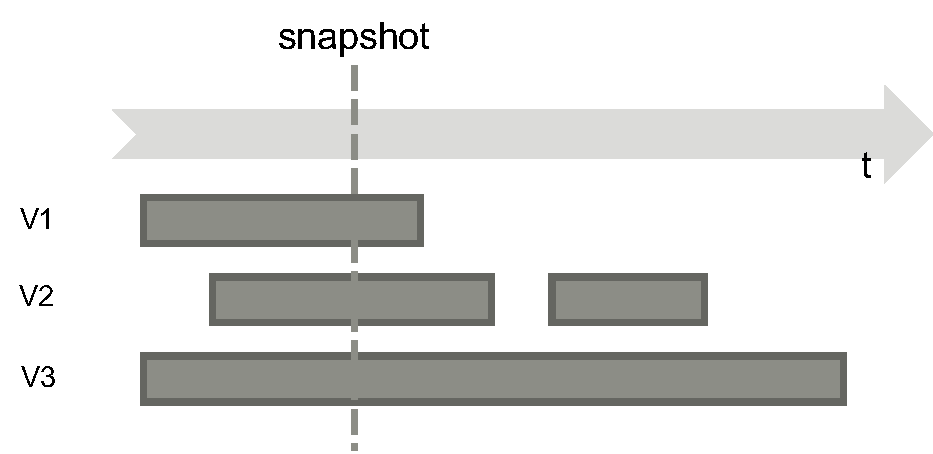
\includegraphics[width=3in]{figs/getsnap.pdf}
\caption{A graph snapshot over interval model TG is a time slice at time t.}
\label{fig:getsnap}
\end{figure}

In our model a snapshot at any time $t$ is state at time $t$ and can
be retrieved by selection on $p$ (Figure~\ref{fig:getsnap}). In SQL
(similarly for E):

\begin{small}
\begin{verbatim}
SELECT *
FROM V
WHERE eperiod CONTAINS DATE ':date';
\end{verbatim}
\end{small}

Another commonly used model is a change stream model~\cite{?}.  In
this model a stream $S$ emits a sequence of graph change events $e$,
each associated with a time $t$ at which it was emitted.  An event can
be of entity creation, deletion, or change in the value of one of the
entity attributes.  Multiple events may be associated with one time
instance and the event emit rate is not constant.

\begin{figure}
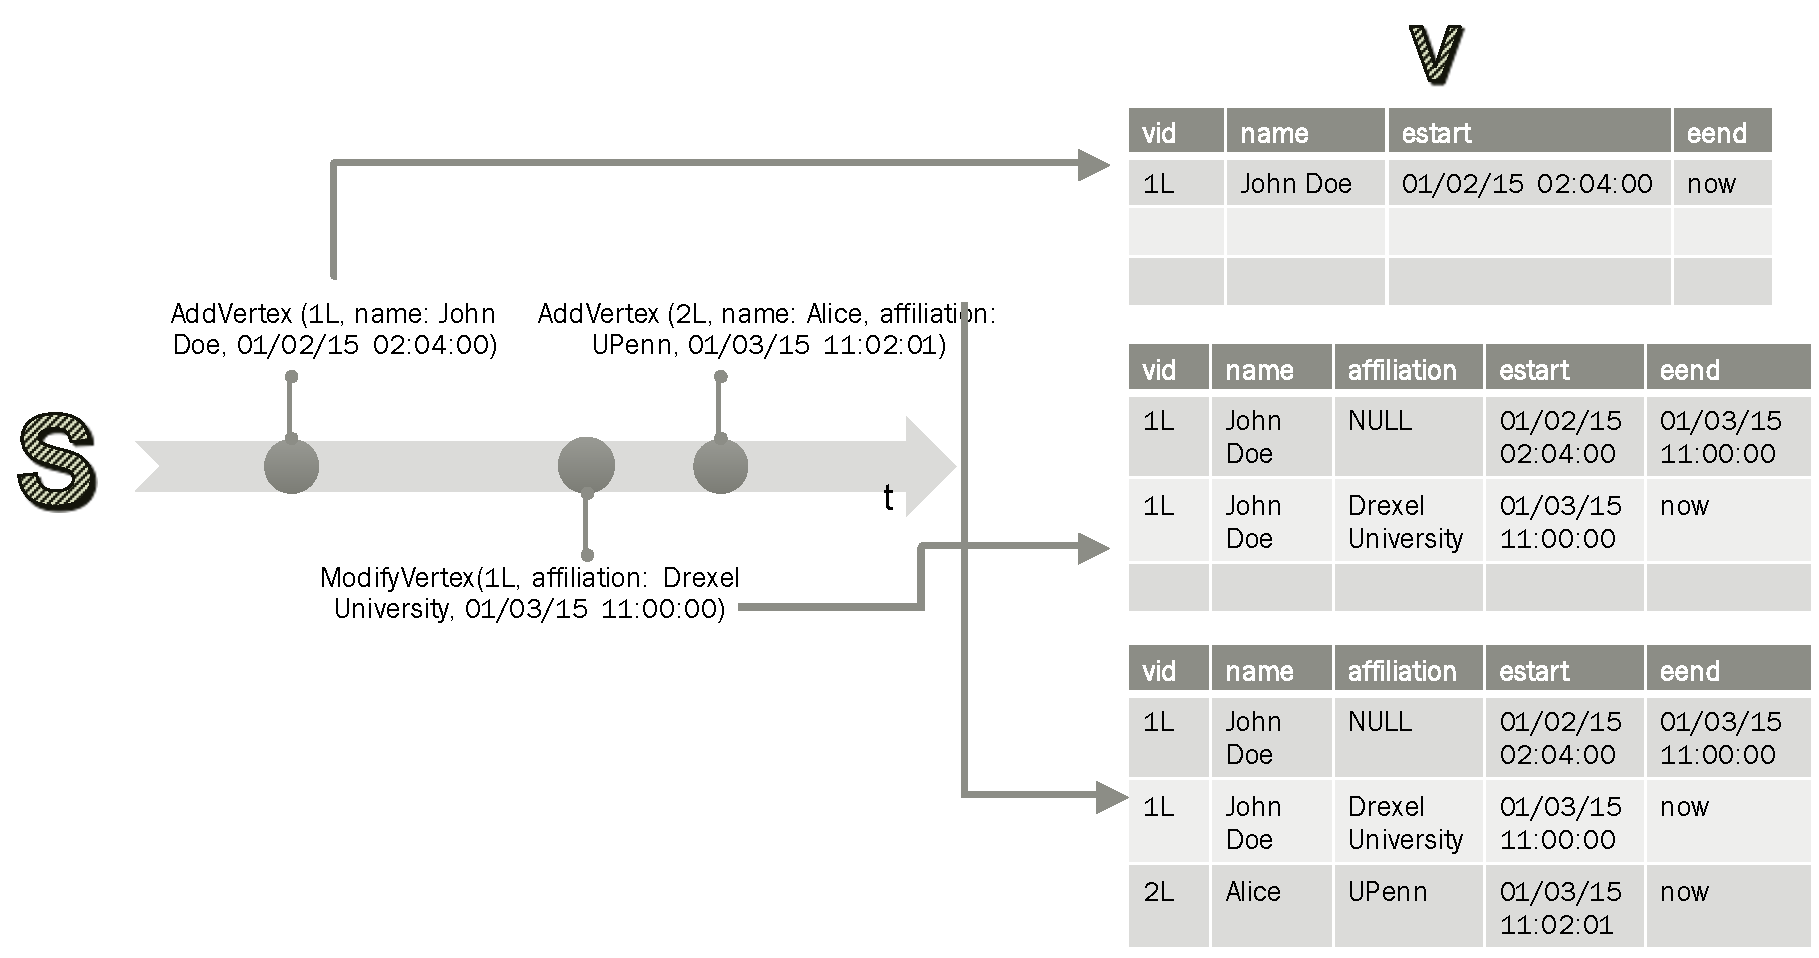
\includegraphics[width=6in]{figs/stream_to_state.pdf}
\caption{Stream $S$ emits graph change events which are converted to
  evolving graph state model $TG$.}
\label{fig:streamtotg}
\end{figure}

Because the stream emits {\em individual entities} rather than {\em
  whole graphs}, graph snapshots can only be reconstructed by
maintaining the history of changes over time.  Our evolving graph
model can be easily constructed from the change stream model following
the conventional temporal database approach
(Figure~\ref{fig:streamtotg}):
\begin{itemize}[noitemsep,topsep=0pt]
\item For an Add event at time $t_i$, add a new tuple with $p=[t_i,
  now)$
\item For a Delete event at time $t_i$, modify the tuple matching the
  primary key by setting $p=[t_s, now)$ to $[t_s, t_i)$.
\item For a Change event at time $t_i$, modify the tuple matching the
  primary key as for a Delete event, and add a new tuple with the
  changed value as for an Add event.
\end{itemize}

This approach assumes that no events arrive out of order and there are
no redundant or duplicate events.  However, it would be a simple
extension to relax these two assumptions.  We also use a closed world
assumption -- if no event is recorded, for our purposes it did not
occur.

\subsection{Algebra}
\label{sec:model:algebra}

All operations in our model take one or two \tgs and return a \tg,
i.e. the algebra is compositional.  More importantly, all operations
maintain the integrity of the model by computing the value of $V$,
followed by the value of $E$, maintaining the foreign key constraint
from $E$ to $V$ and the maximally condensed non-overlapping time
period contraint on both $V$ and $E$.
